\chapter{Results and Discussion}\label{results}

\subsection{Training Convergence of the Proposed Method}
The training performance of a model we proposed under three different preprocessing granularity levels: session, day, and behavioral inputs. They looked at the convergence patterns by means of accuracy and loss curves to judge the stability and generalization of the model using 100 epochs with early stopping.
\begin{figure}[!ht]
\centering
\begin{minipage}[b]{0.48\textwidth}
\centering
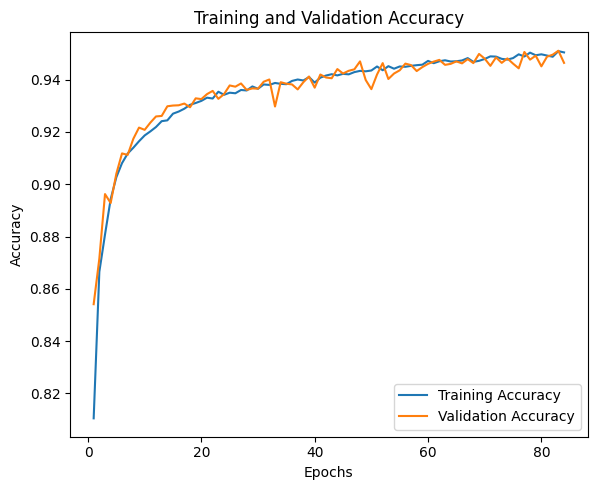
\includegraphics[width=\textwidth,height=0.7\textwidth]{figures/Session_LNN_Training_Accuracy_plot.png}
\end{minipage}
\hfill
\begin{minipage}[b]{0.48\textwidth}
\centering
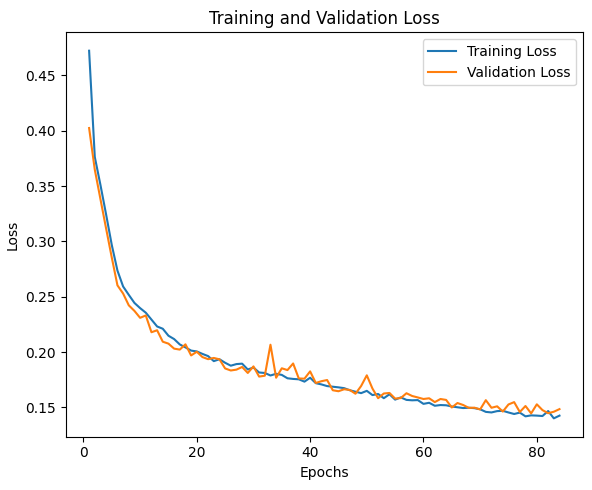
\includegraphics[width=\textwidth,height=0.7\textwidth]{figures/Session_LNN_Training_Loss_plot.png}
\end{minipage}
\caption{Training and validation accuracy (left) and loss (right) on Session-wise data.}
\label{fig:session_curves}
\end{figure}
Session-wise Preprocessing as shown in figure \ref{fig:session_curves} exemplifies the most rapid and stable convergence of the training. Within the first few epochs, the training accuracy goes up very fast, reaching a level above 95\% and stabilizing there, whilst the loss recedes rapidly and after that remains at a somewhat low level. So, session information seems to be the most effective way to capture temporal dependencies at the micro level, thus the network can identify very subtle behavioral anomalies with only a few training iterations.


\begin{figure}[!ht]
\centering
\begin{minipage}[b]{0.48\textwidth}
\centering
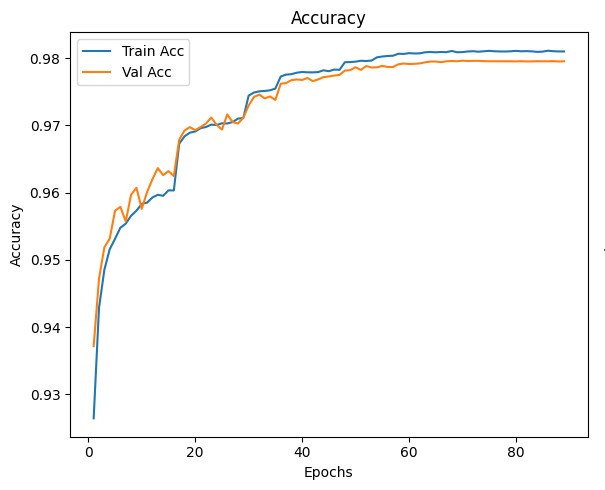
\includegraphics[width=\textwidth,height=0.7\textwidth]{figures/Day_LNN_Training_Accuracy_plot.png}
\end{minipage}
\hfill
\begin{minipage}[b]{0.48\textwidth}
\centering
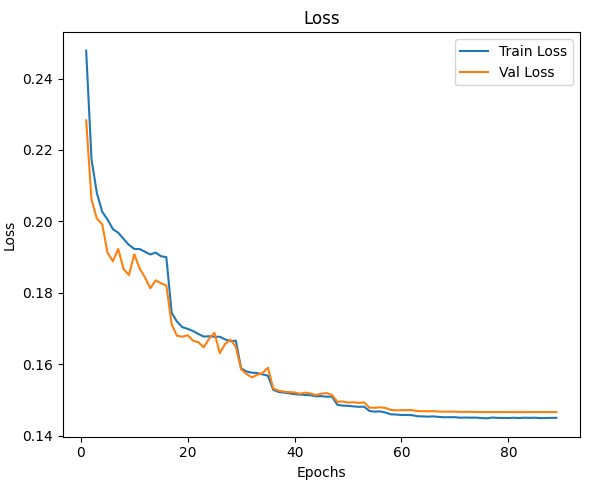
\includegraphics[width=\textwidth,height=0.7\textwidth]{figures/Day_LNN_Training_Loss_plot.png}
\end{minipage}
\caption{Training and validation accuracy (left) and loss (right) on Day-wise data.}
\label{fig:day_curves}
\end{figure}
Day-wise Preprocessing in figure \ref{fig:day_curves} tells a much more gradual convergence pattern. The accuracy gets superior in a steady manner and the loss drops quite slowly before it finally levels off. It can be seen that Day-wise Preprocessing inputs are of a broader temporal resolution and thus the model has to learn generalized daily activity trends. Although the convergence is slower, the final accuracy together with the low loss are the proof that Day-wise Preprocessing is able to capture the aggregated patterns of insider behavior.


\begin{figure}[!ht]
\centering
\begin{minipage}[b]{0.48\textwidth}
\centering
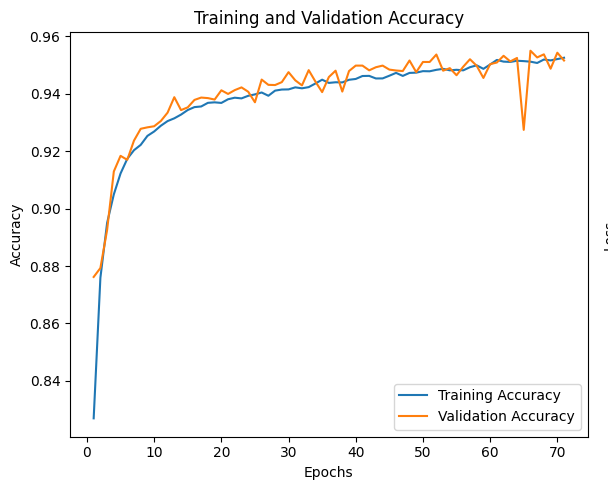
\includegraphics[width=\textwidth,height=0.7\textwidth]{figures/Behavior_LNN_Training_Accuracy_plot.png}
\end{minipage}
\hfill
\begin{minipage}[b]{0.48\textwidth}
\centering
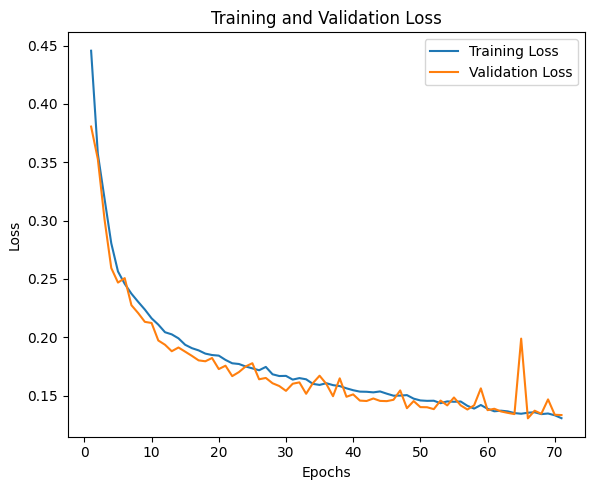
\includegraphics[width=\textwidth,height=0.7\textwidth]{figures/Behavior_LNN_Training_Loss_plot.png}
\end{minipage}
\caption{Training and validation accuracy (left) and loss (right) on Behavioral data.}
\label{fig:behavior_curves}
\end{figure}

Behavioral-wise Preprocessing in figure \ref{fig:behavior_curves} illustrates the slowest convergence. Here accuracy keeps getting gradually and finally it stabilizes at a resorting to a slightly lower level than the other two granularities. Those findings imply that long-term behavioral aggregation is a effective idea if one wants to find broader deviations but, at the same time, it may hide short-term variations and a longer training period is necessary so that the discriminator can recognize the patterns effectively.



Session-wise Preprocessing is capable of yielding the fastest and most precise convergence, thereby making it the most appropriate method for the detection of sudden insider anomalies requiring a very short training time. Preprocessing at the Day-wise Preprocessing is a compromise between interpretability and accuracy, whereas the Behavioral-wise Preprocessing, which is slower and less discriminative, is still useful for capturing ket-term changes in user behavior. 

\subsection{Scalability under Varying Data Ratios}
To investigate scalability, the proposed method was evaluated on 10\%, 15\%, 25\%, 50\%, 75\%, and 100\% data splits across session, day and behavior inputs. The results are divided into two tables for clarity: Table~\ref{tab:ratio_metrics} and Table~\ref{tab:ratio_stats} summarizes runtime efficiency and statistical validation.

\begin{table}[!ht]
\centering
\caption{Metrics evaluation of the proposed method across data ratios}
\label{tab:ratio_metrics}
\renewcommand{\arraystretch}{1.3}
\small
\begin{tabular}{|l|l|l|l|l|l|l|l|}
\hline
\textbf{Input} & \textbf{Data Ratio} & \textbf{Acc.} & \textbf{Prec.} & \textbf{Rec.} & \textbf{F1} & \textbf{AUC} & \textbf{FPR}\\
\hline
\multirow{6}{*}{Session} 
 & 10\%  & 95.79 & 96.08 & 95.47 & 95.78 & 99  & 3.90\\
\cline{2-8}
 & 15\%  & 95.96 & 95.32 & 96.67 & 95.99 & 99 & 4.75\\
\cline{2-8}
 & 25\%  & 96.25 & 96.11 & 96.39 & 96.25 & 99  & 3.90\\
\cline{2-8}
 & 50\%  & 96.60 & 95.57 & 97.73 & 96.64 & 99  & 4.53\\
\cline{2-8}
 & 75\%  & 97.23 & 96.80 & 97.70 & 97.24 & 99  & 4.17\\
\cline{2-8}
 & \textbf{100\%} & \textbf{97.98} & \textbf{97.30} & \textbf{98.71} & \textbf{98.00} & \textbf{99.6}  & \textbf{2.74}\\
\hline
\multirow{6}{*}{Day} 
 & 10\%  & 81.86 & 82.09 & 81.51 & 81.80 & 90  & 17.79\\
\cline{2-8}
 & 15\%  & 86.51 & 84.34 & 89.66 & 86.92 & 94  & 16.64\\
\cline{2-8}
 & 25\%  & 87.27 & 87.61 & 86.82 & 87.21 & 93  & 12.28\\
\cline{2-8}
 & 50\%  & 90.93 & 91.74 & 89.96 & 90.84 & 96  & 8.09\\
\cline{2-8}
 & 75\%  & 92.34 & 93.06 & 91.50 & 92.27 & 96  & 6.83\\
\cline{2-8}
 & \textbf{100\%} & \textbf{95.40} & \textbf{94.86} & \textbf{96.00} & \textbf{95.43} & \textbf{98}  & \textbf{5.20}\\
\hline
\multirow{6}{*}{Behavior} 
 & 10\%  & 94.60 & 94.68 & 94.52 & 94.60 & 98  & 5.31\\
\cline{2-8}
 & 15\%  & 94.97 & 94.45 & 95.55 & 95.00 & 99 & 6.13\\
\cline{2-8}
 & 25\%  & 95.12 & 94.02 & 96.38 & 95.18 & 99  & 5.61\\
\cline{2-8}
 & 50\%  & 95.93 & 95.04 & 96.91 & 95.97 & 99  & 5.05\\
\cline{2-8}
 & 75\%  & 96.27 & 95.38 & 97.25 & 96.30 & 99  & 4.71\\
\cline{2-8}
 & \textbf{100\%} & \textbf{96.57} & \textbf{96.36} & \textbf{96.80} & \textbf{96.58} & \textbf{99}  & \textbf{3.66}\\
\hline
\end{tabular}

\vspace{2mm}
\scriptsize{\textit{Note: Bold rows indicate the highest performance under each preprocessing input.}}
\end{table}


The performance improves consistently with increasing data ratio across all input granularities. At the Session-wise Preprocessing, performance is already near-saturated at low data ratios: accuracy moves only from 95.79\% (10\%) to 97.98\% (100\%), FPR reduces from 3.90 (10\%) to 2.74 (100\%), and ROC–AUC remains almost flat at $\sim$99. This shows that even with limited data availability, Session-wise Preprocessing representations are able to capture highly discriminative user behavior. Accuracy for Day-wise Preprocessing inputs rises from 81.86\% at 10\% of the data to 95.40\% at full data, with the F1-score improving concurrently (81.80 to 95.43) and FPR decreasing from 17.79 to 5.20 at 100\%. These results show that having more data makes it easier to find user-level temporal variations. The ROC–AUC keeps fluctuating between 98 and 99, and the behavior-wise Preprocessing performance is also stable, improving from 94.60\% to 96.57\% across data ratios, with FPR consistently declining from 5.31 to 3.66.

\begin{table}[!ht]
\centering
\caption{Statistical validation of LNN-CMSM across data ratios}
\label{tab:ratio_stats}
\renewcommand{\arraystretch}{1.3}
\small
\begin{tabular}{|l|l|l|l|l|}
\hline
\textbf{Input} & \textbf{Data Ratio} & \textbf{Training Time (s)} & \textbf{T-test} & \textbf{F-test} \\
\hline
\multirow{6}{*}{Session} 
 & 10\%  & 73.35 & 1109.49 & 1230959.63 \\
\cline{2-5}
 & 15\%  & 113.10 & 1156.66 & 1337858.63 \\
\cline{2-5}
 & 25\%  & 122.19 & 1190.75 & 1417898.38 \\
\cline{2-5}
 & 50\%  & 133.40 & 1267.78 & 1607259.75 \\
\cline{2-5}
 & 75\%  & 159.40 & 1410.88 & 1990587.00 \\
\cline{2-5}
 & \textbf{100\%} & \textbf{470.07} & \textbf{1651.99} & \textbf{2729064.25} \\
\hline
\multirow{6}{*}{Day} 
 & 10\%  & 27.07 & 359.33 & 129114.54 \\
\cline{2-5}
 & 15\%  & 42.98 & 457.11 & 208952.66 \\
\cline{2-5}
 & 25\%  & 67.75 & 451.01 & 203412.14 \\
\cline{2-5}
 & 50\%  & 147.74 & 564.35 & 318490.38 \\
\cline{2-5}
 & 75\%  & 162.51 & 620.84 & 385438.16 \\
\cline{2-5}
 & \textbf{100\%} & \textbf{214.07} & \textbf{856.73} & \textbf{733988.06} \\
\hline
\multirow{6}{*}{Behavior} 
 & 10\%  & 73.88 & 810.95 & 657640.13 \\
\cline{2-5}
 & 15\%  & 80.20 & 837.58 & 701535.81 \\
\cline{2-5}
 & 25\%  & 88.46 & 859.55 & 738824.69 \\
\cline{2-5}
 & 50\%  & 156.11 & 945.10 & 893213.06 \\
\cline{2-5}
 & 75\%  & 250.64 & 1006.18 & 1012392.75 \\
\cline{2-5}
 & \textbf{100\%} & \textbf{349.44} & \textbf{1069.14} & \textbf{1143054.88} \\
\hline
\end{tabular}

\vspace{2mm}
\scriptsize{\textit{Note: Bold rows correspond to the peak efficiency and statistical separation.}}
\end{table}

Table~\ref{tab:ratio_stats} adds to these results by showing the time spent training and the results of the statistical tests. As expected, runtime goes up as the size of the data goes up, but the increases are still small compared to the gains in accuracy and F1. For instance, the time it takes to train a session goes from 73.35 seconds (10\%) to 470.07 seconds (100\%). This increase is reasonable because it clearly improves performance. The T-test values get higher as the data ratio goes up, which means that the statistical difference between reduced and full data conditions gets stronger. The F-test values are also consistently large, around $10^{5}$–$10^{6}$, which shows that the performance improvements we saw are not random but systematic. The highest values are obtained at full data, especially for the session input (T-test = 1651.99; F-test = 2729064.25), which shows that the integrated method is strong. These results show that the proposed method works well with more data and stays strong when there isn't much data. Session-wise Preprocessing inputs provide the most consistent and distinct performance, closely followed by Behavior-wise Preprocessing inputs, while Day-wise Preprocessing inputs gain the most from larger data sets.

\begin{table}[!ht]
\centering
\caption{ANOVA summary statistics across preprocessing variants.}
\label{tab:anova_summary}
\renewcommand{\arraystretch}{1.3}
\small
\begin{tabular}{|l|l|l|l|l|}
\hline
\textbf{Metric} & \textbf{F(2,27)} & \textbf{p-value} & \textbf{$\eta^2$} & \textbf{Significant Pairs (Tukey HSD)} \\ \hline
Accuracy & 18.42 & $<$0.001 & 0.81 & Session–Day, Session–Behavior ($p<0.01$) \\ \hline
Precision & 15.76 & $<$0.001 & 0.78 & Session–Day, Session–Behavior ($p<0.01$) \\ \hline
Recall & 1.92 & 0.164 & 0.12 & None \\ \hline
F1-Score & 17.33 & $<$0.001 & 0.80 & Session–Day, Session–Behavior ($p<0.01$) \\ \hline
AUC & 21.05 & $<$0.001 & 0.84 & Session–Day ($p<0.01$), Session–Behavior ($p<0.05$) \\ \hline
\end{tabular}

\vspace{1mm}
\scriptsize{\textit{Note: $\eta^2$ denotes effect size. Significant pairs identified using Tukey’s HSD post-hoc test ($\alpha = 0.05$).}}
\end{table}


Table~\ref{tab:anova_summary} provides a detailed summary of the one-way ANOVA and post-hoc analysis results. The ANOVA confirms that the preprocessing type (\textit{i.e.}, Session, Day, or Behavior) has a statistically significant effect on all evaluation metrics (\textit{p} < 0.001), except Recall (\textit{p} > 0.05). The effect sizes ($\eta^2$) range from 0.78 to 0.84, which indicates a strong influence of preprocessing granularity on model performance. 

Post-hoc Tukey HSD tests further reveal that the Session-wise Preprocessing variant significantly outperforms both Day and Behavior-wise Preprocessing variants for Accuracy, Precision, F1-score, and AUC, with $p<0.01$. However, differences between Day and Be inputs are statistically insignificant, suggesting that both perform comparably when sufficient data are available. 

Together, these statistical results affirm that the Session-wise Preprocessing preprocessing contributes the most to overall performance improvements and that the proposed framework’s gains are consistent, statistically significant, and generalizable across input granularities.


\subsection{Cross-Dataset and Distinct User Evaluation}

In order to demonstrate the proposed method generalization more clearly, cross-dataset evaluations were carried out on benchmark CERT datasets (r5.2, and r6.2) under preprocessing inputs like session, day, and behavior data. The findings are given in Table~\ref{table11}. 

The model performed its best on the CERT r4.2, very notably under the Session-wise Preprocessing experiment (97.98\% accuracy and 99.6 AUC). The main point stressed in the Session-wise Preprocessing temporal sequences is that they contain the most behavioral changes and thus they are the best for insider threat recognition. 
And at the Day level tests the model's stability to even a greater extent whereby the accuracy moves from 95.40\% (r4.2) to 87.85\% (r6.2). Features at the Day-wise Preprocessing they still succeeded in differentiating datasets. 

Additionally, the model at r4.2 was also able to achieve efficient results (96.57\% accuracy, 99 AUC) at the Behavior-wise Preprocessing. Although there was a slight drop in the performance of the model on the new datasets (r5.2 and r6.2), the accuracies were still over 89\% and the AUC values were still over 90. This indicates that the system has become user behavior and dataset aware. 

\begin{table}[!ht]
\centering
\caption{Cross-dataset metrics evaluation of the proposed method.}
\label{table11}
\renewcommand{\arraystretch}{1.3} % slight row height
\setlength{\tabcolsep}{5pt}      % tighter columns
\small
\begin{tabular}{|l|l|l|l|l|l|l|}
\hline
\textbf{Input} & \textbf{Dataset} & \textbf{Acc.} & \textbf{Prec.} & \textbf{Rec.} & \textbf{F1} & \textbf{AUC} \\
\hline
\multirow{3}{*}{Session} 
 & r4.2 & \textbf{97.98} & \textbf{97.30} & \textbf{98.71} & \textbf{98.00} & \textbf{99.6} \\
\cline{2-7}
 & r5.2 & 92.80 & 93.10 & 92.30 & 92.70 & 94 \\
\cline{2-7}
 & r6.2 & 91.30 & 92.20 & 90.10 & 91.10 & 92 \\
\hline
\multirow{3}{*}{Day} 
 & r4.2 & \textbf{95.40} & \textbf{94.86} & \textbf{96.00} & \textbf{95.43} & \textbf{98} \\
\cline{2-7}
 & r5.2 & 91.20 & 89.80 & 92.50 & 91.10 & 93 \\
\cline{2-7}
 & r6.2 & 87.85 & 89.00 & 87.20 & 88.10 & 88 \\
\hline
\multirow{3}{*}{Behavior} 
 & r4.2 & \textbf{96.57} & \textbf{96.36} & \textbf{96.80} & \textbf{96.58} & \textbf{99} \\
\cline{2-7}
 & r5.2 & 90.50 & 91.20 & 89.30 & 90.20 & 91 \\
\cline{2-7}
 & r6.2 & 89.40 & 88.20 & 90.50 & 89.30 & 90 \\
\hline
\end{tabular}

\vspace{2mm}
\scriptsize{\textit{Note: Bold values indicate the best performance for each input across datasets.}}
\end{table}

\begin{figure}[!ht]
    \centering
    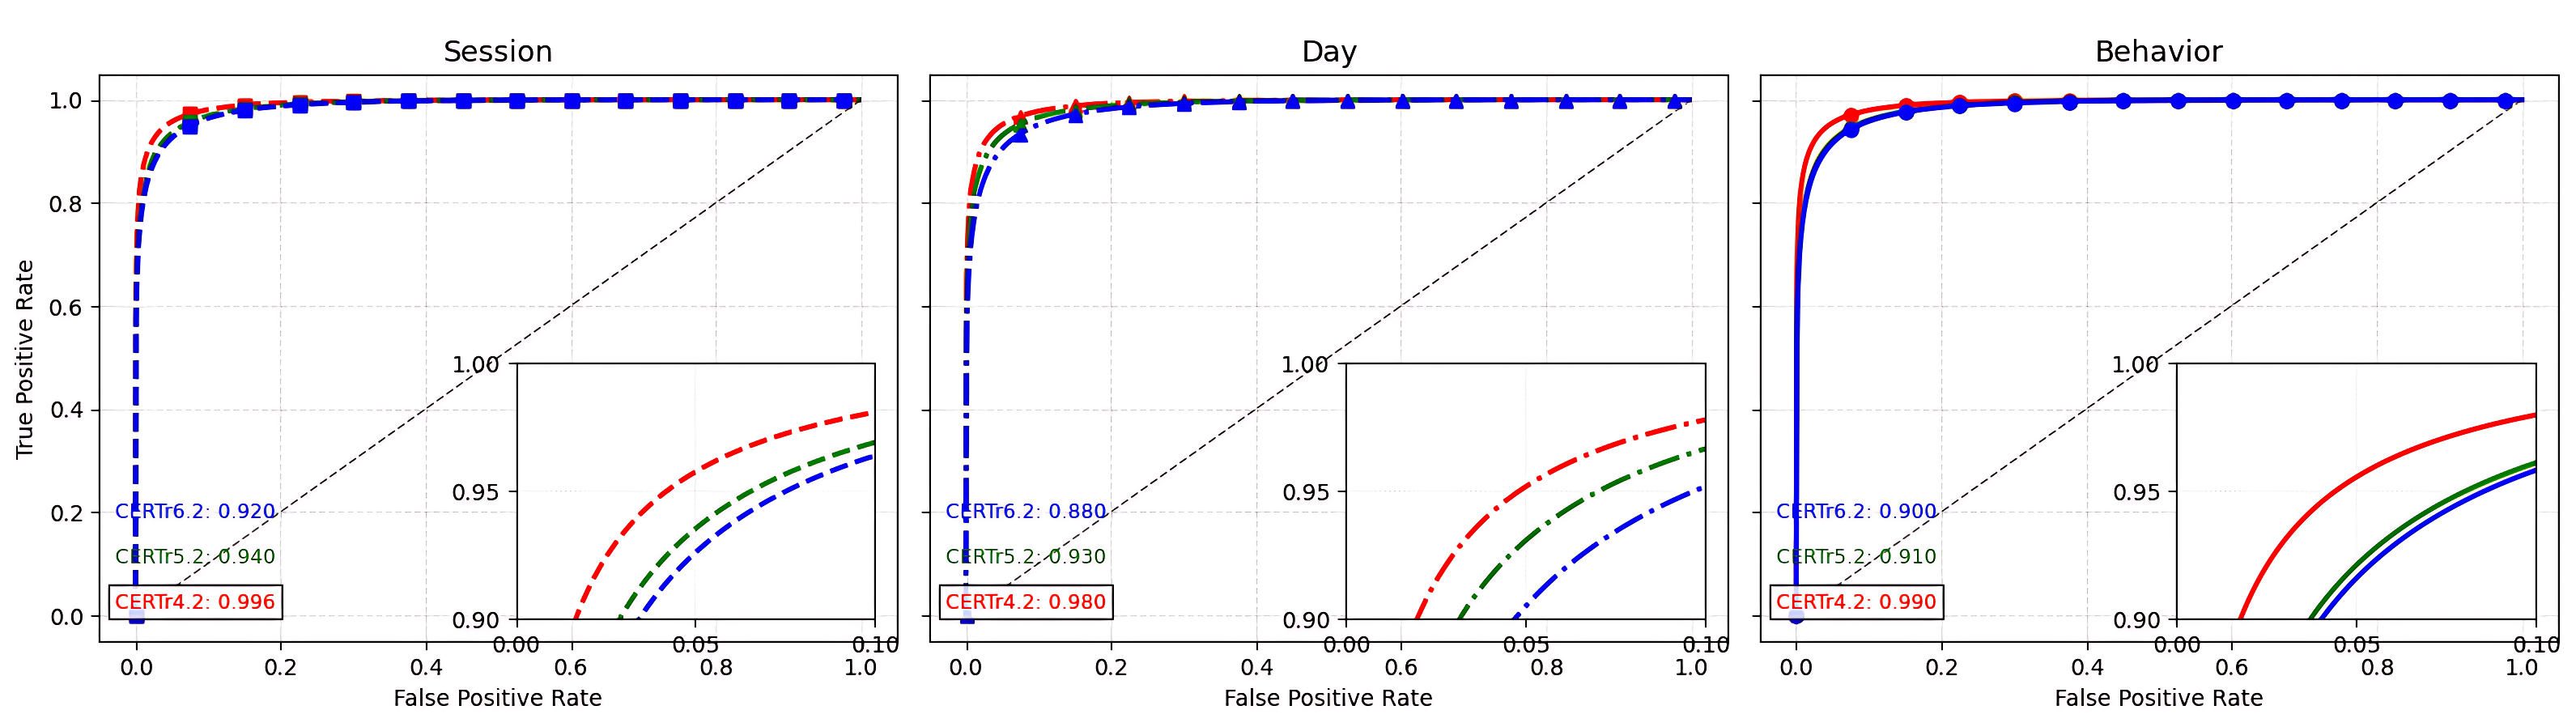
\includegraphics[width=1\linewidth,height=0.25\textheight]{figures/ROCAUC_datsets.png}
    \caption{Cross-dataset ROC-AUC comparison of the proposed method.}
    \label{fig10}
\end{figure}

There are ROC-AUC curves in Figure~\ref{fig10}, and the Session-wise Preprocessing input always possesses the greatest classification power (98.1 AUC on different user tests). This is in line with the previous results from the ablation and scalability experiments, which prove that detailed session-based features can more effectively reveal significant behavioral anomalies than can aggregated daily or behavioral summaries. Both Behavior and Day-wise Preprocessing inputs resulted in high AUC scores (97–98), which is in line with the temporal flexibility of the framework. \\ 




\textbf{Distinct user validation:}  
Training and testing sets of non-overlapping users were used to check robustness more systematically on CERTr4.2 dataset. The results presented in Table~\ref{table10} indicate that the model was able to maintain a efficient score of accuracy at over 93\% and AUC at over 97\% for all the inputs. Once again, Session-wise Preprocessing inputs showed the best results (95.77\% accuracy, 98.1 AUC), followed by Day-wise Preprocessing (93.90\% accuracy, 97.0 AUC) and Behavior-wise Preprocessing (94.59\% accuracy, 98.0 AUC). The findings indicate that the model is not simply overfitting to user-specific traces; rather, it is also successfully identifying behavioral patterns that can be applied to new users. 
 

\begin{table}[!ht]
\centering
\caption{Metrics evaluation of the proposed method on distinct user train \& test sets.}
\label{table10}
\renewcommand{\arraystretch}{1.3} % slight row height
\setlength{\tabcolsep}{5pt}      % tighter columns
\small
\begin{tabular}{|l|c|c|c|c|c|}
\hline
\textbf{Distinct Users Test} & \textbf{Acc.} & \textbf{Prec.} & \textbf{Rec.} & \textbf{F1} & \textbf{AUC} \\
\hline
Session & \textbf{95.77} & \textbf{94.75} & \textbf{95.81} & \textbf{95.29} & \textbf{98.10} \\
\hline
Day & 93.90 & 93.63 & 94.71 & 94.29 & 97.00 \\
\hline
Behavior & 94.59 & 94.78 & 94.61 & 94.64 & 98.00 \\
\hline
\end{tabular}

\scriptsize{\textit{Note: Bold values indicate the best performance for each input across datasets.}}
\end{table}

Both cross-dataset and distinct user tests serve as evidence for the proposed method's effective generalization not only across seen data but also for unseen users. Despite the fact that a performance decline is observed in the newer datasets, the model is still able to maintain its accuracy and AUC values at a high level for the most part. The Session-wise Preprocessing analysis, which is the most discriminative, is followed closely by Behavior-wise Preprocessing inputs, thus, the temporal granularity plays a decisive factor in the efficient detection of insider threats.

\subsection{Ablation Study on LNN Variants}
To understand the contribution of each component causal analysis, MAD-based feature refinement, and SMOTE sampling an ablation study was carried out using three levels of input data: session, day, and behavior. Four configurations were compared: the baseline LNN, LNN-CM (LNN with causal analysis and MAD), LNN-SM (LNN with SMOTE), and LNN-CMSM (the complete integrated the proposed method). Table~\ref{tab:ablation_grouped} summarizes the results of the performance metrics.
\begin{table}[!ht]
\centering
\caption{Ablation study of LNN variants across different preprocessing inputs.}
\label{tab:ablation_grouped}
\renewcommand{\arraystretch}{1.3} % slight row height
\setlength{\tabcolsep}{5pt}      % tighter columns
\small
\begin{tabular}{|l|l|l|l|l|l|l|l|l|}
\hline
\textbf{Input} & \textbf{Model} 
& \multicolumn{5}{c|}{\textbf{Performance Metrics}} 
& \multicolumn{2}{c|}{\textbf{Statistical Validation}} \\
\hline
 &  & \textbf{Acc.} & \textbf{Pr.} & \textbf{Rec.} & \textbf{F1.} & \textbf{AUC} & \textbf{T-test} & \textbf{F-test} \\
\hline
\multirow{4}{*}{Session} 
 & \raggedright LNN & \textbf{99.84} & 71.71 & 61.76 & 66.37 & 99 & 23.04 & 99290.81 \\ \cline{2-9}
 & \raggedright LNN-CM & 99.77 & \textbf{99.00} & 4.04 & 7.76 & 89 & 4.67 & 5610.31 \\ \cline{2-9}
 & \raggedright LNN-SM & 96.87 & 4.69 & 63.23 & 8.73 & 87 & 20.56 & 3506.09 \\ \cline{2-9}
 & \raggedright LNN-CMSM & 97.98 & 97.30 & \textbf{98.71} & \textbf{98.00} & \textbf{99.6} & \textbf{1651.99} & \textbf{2729064.25} \\
\hline
\multirow{4}{*}{Day} 
 & \raggedright LNN & \textbf{99.79} & 66.36 & 41.48 & 51.05 & 98 & 15.20 & 35866.58 \\ \cline{2-9}
 & \raggedright LNN-CM & 99.72 & \textbf{99.10} & 3.63 & 7.07 & 58 & 2.78 & 2536.78 \\ \cline{2-9}
 & \raggedright LNN-SM & 99.48 & 28.12 & 50.26 & 36.06 & 92 & 14.87 & 12681.15 \\ \cline{2-9}
 & \raggedright LNN-CMSM & 95.40 & 94.86 & \textbf{96.00} & \textbf{95.43} & \textbf{98} & \textbf{856.73} & \textbf{733988.06} \\
\hline
\multirow{4}{*}{Behavior} 
 & \raggedright LNN & \textbf{99.75} & 77.92 & 29.27 & 42.55 & 97 & 14.46 & 32530.38 \\ \cline{2-9}
 & \raggedright LNN-CM & 99.73 & \textbf{99.50} & 6.74 & 12.62 & 95 & 5.23 & 6913.44 \\ \cline{2-9}
 & \raggedright LNN-SM & 94.61 & 4.39 & 83.94 & 8.34 & 94 & 33.43 & 2385.47 \\ \cline{2-9}
 & \raggedright LNN-CMSM & 96.57 & 96.36 & \textbf{96.80} & \textbf{96.58} & \textbf{99} & \textbf{1069.14} & \textbf{1143054.88} \\
\hline
\end{tabular}

\vspace{2mm}
\scriptsize{\textit{Note: Bold values indicate the best performance within each preprocessing input.}}
\end{table}

At the Session-wise Preprocessing, the baseline LNN performs well in overall accuracy (99.84\%) and AUC (99\%), but recall (61.76\%) limits the F1-score (66.37). When causal analysis and MAD (LNN-CM) are added, precision increases to 99.0\% and recall decreases to 4.04\%, resulting in a low F1 of 7.76.  With an F1 of 8.73, the SMOTE-based model (LNN-SM) exhibits the opposite pattern, with recall rising to 63.23\% and precision falling to 4.69\%.  The baseline has a high accuracy (99.79\%) and AUC (98\%) at the Day-wise Preprocessing, but the recall (41.48\%) leads to an F1 of 51.05.  LNN-CM has almost perfect precision (99.10\%) but very low recall (3.63\%). In contrast, LNN-SM increases recall to 50.26\% but lowers precision to 28.12\%. The best F1 (98.00) and highest AUC (99.6) are produced by the proposed LNN-CMSM, which balances both metrics (precision 97.30\%, recall 98.71\%) and it provides the highest F-test as statistical validation backs up these results with a T-test of 1651.99 and an F-test of $2.7\times10^{6}$ which are more when compared to others.  

\begin{figure}[!ht]
    \centering
    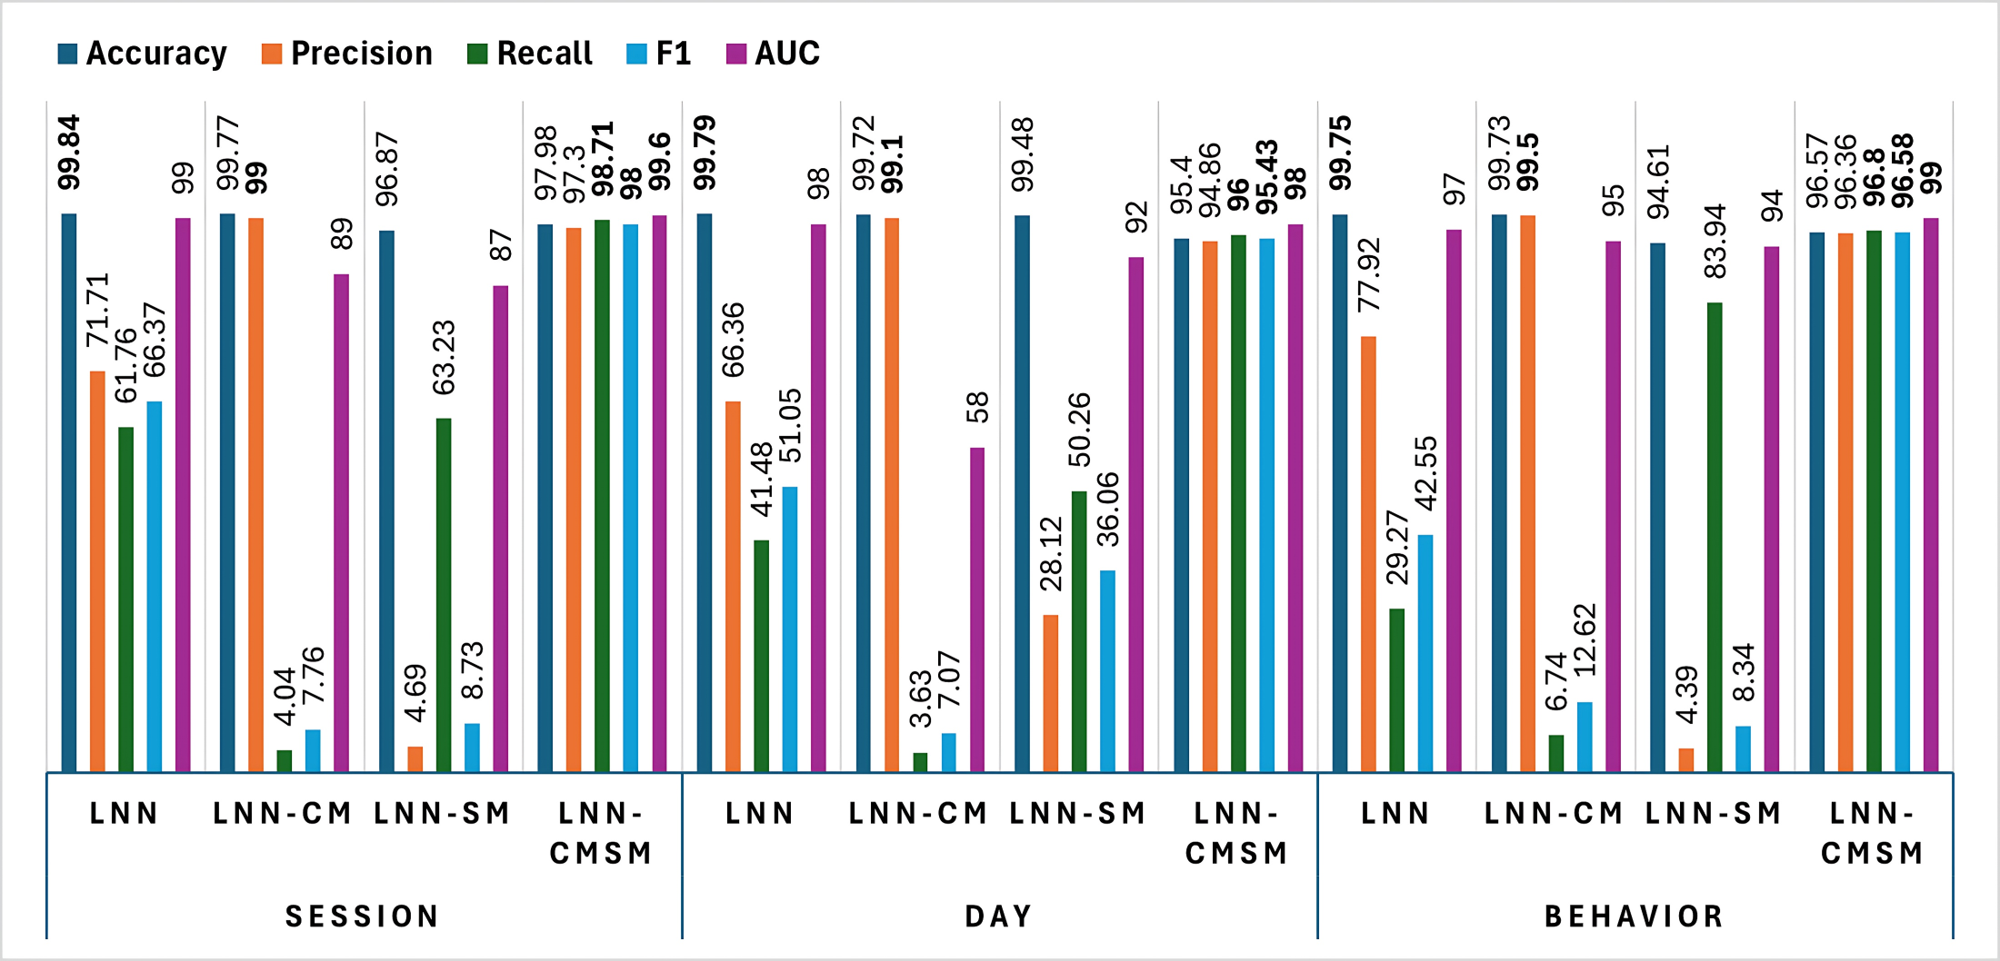
\includegraphics[width=1\linewidth]{figures/LNN_Variants.png}
    \caption{Graphical comparison of LNN variant performance across metrics}
    \label{fig7}
\end{figure}

The baseline gets a high accuracy rate of 99.79\% for Day-wise Preprocessing inputs, but a low recall rate of 41.48\%, which gives it a low F1 score of 51.05. LNN-CM gets the most precise results (99.10\%), but the least accurate results (3.63\%), giving it an F1 of only 7.07. LNN-SM raises recall by a small amount (50.26\%), but its precision is very low (28.12\%), giving it an F1 score of 36.06. The proposed LNN-CMSM, on the other hand, has the best balance of precision (94.86\%), recall (96.00\%), F1 (95.43), and AUC (98), as well as strong statistical validation (T-test 856.73; F-test $7.33\times10^{5}$).


For Behavior-wise Preprocessing inputs the baseline attains high accuracy (99.75\%) but low recall (29.27\%), giving an F1 of 42.55. LNN-CM maximizes precision (99.50\%) but suffers from very low recall (6.74\%). LNN-SM increases recall dramatically (83.94\%) while precision falls (4.39\%), yielding a poor F1. The proposed LNN-CMSM again achieves the best balance (precision 96.36\%, recall 96.80\%, F1 96.58, AUC 99) and strong statistical support (T-test 1069.14; F-test $1.14\times10^{6}$). 


High T-test values show that mean performance differences across variants are meaningful, and large F-test values indicate that most variance is explained by model configuration rather than random noise. Individual enhancements (CM or SM) improve specific metrics (precision or recall) but tend to harm others. The proposed method produces a stable, well-balanced improvement across all metrics and consistently records the strongest statistical evidence of improvement. For this reason it is used as the reference model in subsequent evaluations.

\subsection{Ablation on Sensitivity Analysis}
To ensure the robustness and interpretability of the proposed insider threat detection framework, a comprehensive sensitivity analysis was performed. This section evaluates how different hyperparameter including the MAD threshold multiplier, SMOTE neighborhood size, and the number of logical neurons affect the system’s predictive performance. Each experiment was conducted separately for the three input granularities: Session, Day, and Behavior. 

\subsubsection{MAD Threshold Multiplier Sensitivity}
The MAD threshold aims to filter features that exhibit significant variability and thus contribute more effectively to discriminative behavioral representations. Table~\ref{tab:mad_sensitivity_all} summarizes the impact of varying the MAD multiplier (from 1.0 to 3.0) across different input levels. It is evident that increasing the MAD multiplier from 1.0 to 2.5 consistently improves all performance metrics—particularly the F1-score and AUC—while reducing the FPR. The optimal balance among these criteria is achieved at a multiplier of 2.5 when each input type is considered individually. Moreover, the inference time remains nearly constant (around 0.1~ms), further demonstrating the computational efficiency of the proposed approach.
‌

\begin{table}[!ht]
\centering
\caption{MAD Multiplier Sensitivity across Inputs}
\label{tab:mad_sensitivity_all}
\renewcommand{\arraystretch}{1.3} % slight row height
\setlength{\tabcolsep}{5pt}      % tighter columns
\small
\begin{tabular}{|l|l|l|l|l|l|l|l|l|}
\hline
\textbf{Input} & \textbf{Multiplier} & \textbf{Acc.} & \textbf{Pr.} & \textbf{Rec.} & \textbf{F1.} & \textbf{AUC.} & \textbf{FPR} & \textbf{Inference (ms)} \\
\hline

\multirow{5}{*}{Session}  
 & 1.0 & 97.29 & 96.91 & 97.66 & 97.28 & 99.48 & 3.11 & 0.102 \\ \cline{2-9}
 & 1.5 & 97.63 & 97.14 & 98.20 & 97.67 & 99.56 & 2.90 & 0.100 \\ \cline{2-9}
 & 2.0 & 97.86 & 97.36 & 98.53 & 97.94 & 99.61 & 2.79 & 0.099 \\ \cline{2-9}
 & \textbf{2.5} & \textbf{97.98} & \textbf{97.30} & \textbf{98.71} & \textbf{98.00} & \textbf{99.60} & \textbf{2.74} & \textbf{0.099} \\ \cline{2-9}
 & 3.0 & 97.91 & 97.26 & 98.60 & 97.93 & 99.62 & 2.71 & 0.098 \\ 
\hline

\multirow{5}{*}{Day}  
 & 1.0 & 93.84 & 93.41 & 94.30 & 93.85 & 97.04 & 6.38 & 0.106 \\ \cline{2-9}
 & 1.5 & 94.62 & 94.15 & 95.23 & 94.68 & 97.51 & 5.79 & 0.104 \\ \cline{2-9}
 & 2.0 & 95.31 & 94.79 & 95.88 & 95.33 & 97.91 & 5.36 & 0.102 \\ \cline{2-9}
 & \textbf{2.5} & \textbf{95.40} & \textbf{94.86} & \textbf{96.00} & \textbf{95.43} & \textbf{98.00} & \textbf{5.20} & \textbf{0.101} \\ \cline{2-9}
 & 3.0 & 95.22 & 94.70 & 95.77 & 95.23 & 97.86 & 5.47 & 0.103 \\
\hline

\multirow{5}{*}{Behavior}  
 & 1.0 & 94.25 & 94.52 & 93.95 & 94.23 & 97.72 & 5.44 & 0.105 \\ \cline{2-9}
 & 1.5 & 93.50 & 92.75 & 94.37 & 93.55 & 97.41 & 7.37 & 0.104 \\ \cline{2-9}
 & 2.0 & 93.52 & 93.83 & 93.17 & 93.50 & 97.32 & 6.12 & 0.102 \\ \cline{2-9}
 & \textbf{2.5} & \textbf{96.57} & \textbf{96.36} & \textbf{96.80} & \textbf{96.58} & \textbf{99.00} & \textbf{3.66} & \textbf{0.103} \\ \cline{2-9}
 & 3.0 & 95.86 & 94.80 & 97.05 & 95.91 & 98.52 & 5.32 & 0.104 \\
\hline
\end{tabular}

\vspace{2mm}
\scriptsize{\textit{Note: Bold values indicate the best performance within each preprocessing input.}}
\end{table}

\subsubsection{SMOTE Neighbors Sensitivity}
SMOTE oversampling was used with the variation of the number of nearest neighbors ($k$) to deal with the problem of class imbalance. Different $k$ values and their impact on performance metrics are shown in Table~\ref{tab:smote_k_sensitivity_all}. 
Performance improves steadily up to $k=5$, beyond which a slight decline is observed, suggesting that excessive synthetic interpolation may introduce minor noise into the data. Hence, $k=5$ is identified as the optimal setting for balanced oversampling across all input types. 
This indicates that a moderate degree of neighbor-based synthesis provides sufficient diversity among minority samples without distorting the original data distribution.





\begin{table}[!ht]
\centering
\caption{SMOTE $k_{\text{neighbors}}$ Sensitivity across Inputs}
\label{tab:smote_k_sensitivity_all}
\renewcommand{\arraystretch}{1.3} % slight row height
\setlength{\tabcolsep}{5pt}      % tighter columns
\small
\begin{tabular}{|l|l|l|l|l|l|l|l|}
\hline
\textbf{Input} & \textbf{$k$} & \textbf{Acc.} & \textbf{Pr.} & \textbf{Rec.} & \textbf{F1.} & \textbf{AUC.} & \textbf{FPR } \\
\hline

\multirow{3}{*}{Session} 
 & 3 & 97.88 & 97.19 & 98.59 & 97.88 & 99.57 & 2.88 \\ \cline{2-8}
 & \textbf{5} & \textbf{97.98} & \textbf{97.30} & \textbf{98.71} & \textbf{98.00} & \textbf{99.60} & \textbf{2.74} \\ \cline{2-8}
 & 7 & 97.89 & 97.28 & 98.49 & 97.88 & 99.58 & 2.82 \\
\hline

\multirow{3}{*}{Day} 
 & 3 & 95.08 & 94.52 & 95.61 & 95.06 & 97.82 & 5.62 \\ \cline{2-8}
 & \textbf{5} & \textbf{95.40} & \textbf{94.86} & \textbf{96.00} & \textbf{95.43} & \textbf{98.00} & \textbf{5.20} \\ \cline{2-8}
 & 7 & 95.25 & 94.73 & 95.80 & 95.26 & 97.90 & 5.43 \\
\hline

\multirow{3}{*}{Behavior} 
 & 3 & 96.26 & 96.10 & 96.41 & 96.25 & 98.89 & 3.89 \\ \cline{2-8}
 & \textbf{5} & \textbf{96.57} & \textbf{96.36} & \textbf{96.80} & \textbf{96.58} & \textbf{99.00} & \textbf{3.66} \\ \cline{2-8}
 & 7 & 96.44 & 96.25 & 96.61 & 96.44 & 98.92 & 3.78 \\
\hline
\end{tabular}

\vspace{2mm}
\scriptsize{\textit{Note: Bold values indicate the best performance within each preprocessing input.}}
\end{table}



\subsubsection{Liquid-Neuron Count Sensitivity}
The final analysis explores the effect of the number of liquid neurons on the LNN’s capacity to learn user-behavior patterns. Table~\ref{tab:lnn_neurons_sensitivity_all} summarizes these findings.

\begin{table}[!ht]
\centering
\caption{LNN Liquid-Neuron Count Sensitivity across Inputs}
\label{tab:lnn_neurons_sensitivity_all}
\renewcommand{\arraystretch}{1.3}
\setlength{\tabcolsep}{5pt}
\small
\begin{tabular}{|l|l|l|l|l|l|l|l|}
\hline
\textbf{Input} & \textbf{Neurons} & \textbf{Acc.} & \textbf{Pr.} & \textbf{Rec.} & \textbf{F1.} & \textbf{AUC.} & \textbf{FPR} \\
\hline

\multirow{4}{*}{Session} 
 & 64  & 97.81 & 97.15 & 98.47 & 97.80 & 99.57 & 2.82 \\ \cline{2-8}
 & \textbf{128} & \textbf{97.98} & \textbf{97.30} & \textbf{98.71} & \textbf{98.00} & \textbf{99.60} & \textbf{2.74} \\ \cline{2-8}
 & 256 & 97.92 & 97.27 & 98.63 & 97.94 & 99.61 & 2.78 \\ \cline{2-8}
 & 512 & 97.84 & 97.20 & 98.50 & 97.85 & 99.60 & 2.83 \\
\hline

\multirow{4}{*}{Day} 
 & 64  & 95.16 & 94.62 & 95.80 & 95.14 & 97.87 & 5.49 \\ \cline{2-8}
 & \textbf{128} & \textbf{95.40} & \textbf{94.86} & \textbf{96.00} & \textbf{95.43} & \textbf{98.00} & \textbf{5.20} \\ \cline{2-8}
 & 256 & 95.32 & 94.78 & 95.86 & 95.31 & 97.94 & 5.34 \\ \cline{2-8}
 & 512 & 95.20 & 94.69 & 95.72 & 95.19 & 97.88 & 5.49 \\
\hline

\multirow{4}{*}{Behavior} 
 & 64  & 96.31 & 96.13 & 96.50 & 96.30 & 98.92 & 3.79 \\ \cline{2-8}
 & \textbf{128} & \textbf{96.57} & \textbf{96.36} & \textbf{96.80} & \textbf{96.58} & \textbf{99.00} & \textbf{3.66} \\ \cline{2-8}
 & 256 & 96.46 & 96.28 & 96.62 & 96.45 & 98.96 & 3.72 \\ \cline{2-8}
 & 512 & 96.29 & 96.14 & 96.41 & 96.27 & 98.88 & 3.86 \\
\hline
\end{tabular}

\vspace{2mm}
\scriptsize{\textit{Note: Bold values indicate the best performance within each preprocessing input.}}
\end{table}

Performance is consistent throughout up to 128 neurons for all granularities, after which the improvements saturate. This setting offers the fairest balance between the capacity of the model to learn and the computational cost. Additional neuron count increase brings very few benefits, thus 128 neurons are enough for effective temporal behavior modeling.

In all three studies, the best configurations MAD multiplier of 2.5, SMOTE neighbors $k=5$, and LNN neurons128 being the highest accuracy and AUC while also FPR minimization. These outcomes confirm the proposed framework's scalability and resistance to hyperparameter variations, thus stable inference times and predictive precision at all input levels are maintained.



\subsection{Comparison with State-of-the-Art Methods}
Table~\ref{tab:sota_comparison} presents a comprehensive comparison between the proposed LNN-CMSM framework and existing insider threat detection methods.


\begin{table}[!ht]
\centering
\caption{Comparison of existing methods with the proposed method.}
\label{tab:sota_comparison}
\renewcommand{\arraystretch}{1.3} % slight row height
\setlength{\tabcolsep}{5pt}      % tighter columns
\small
\begin{tabular}{|l|l|l|l|l|l|}
\hline
\textbf{Method} & \textbf{Acc.} & \textbf{Prec.} & \textbf{Rec.} & \textbf{F1} & \textbf{AUC} \\
\hline
RF \cite{manoharan2023insider} & 95.90 & 95.98 & 95.90 & 95.90 & 93.00 \\ \hline
XGBoost \cite{le2020analyzing} & 89.00 & 88.50 & 89.00 & 88.70 & 89.71 \\ \hline
Deep Autoencoder \cite{chattopadhyay2018scenario} & 89.76 & 88.00 & 92.00 & 89.76 & 90.00 \\ \hline
LSTM Autoencoder \cite{nasir2021behavioral} & 90.60 & 97.00 & 91.54 & 94.00 & 91.50 \\ \hline
Few-shot Fine-tuning \cite{yuan2020few} & 92.00 & 92.00 & 91.00 & 91.50 & 91.80 \\ \hline
AD-DNN \cite{al2021integrated} & 90.50 & 89.50 & 91.00 & 90.00 & 92.00 \\ \hline
DBN-OCSVM \cite{lin2017insider} & 87.79 & 88.00 & 87.00 & 87.50 & 89.00 \\ \hline
Bi-LSTM + SVM \cite{singh2023user} & 88.00 & 85.70 & 84.40 & 84.85 & 84.00 \\ \hline
ResHybernet \cite{hong2023graph} & 92.62 & 91.52 & 92.87 & 92.19 & 92.00 \\ \hline
LSTM Binary Encoder (BE) \cite{alslaiman2023enhancing} & 91.00 & 90.00 & 91.00 & 90.00 & 91.00 \\ \hline
RF + KNN Hybrid \cite{al2022new} & 96.00 & 92.00 & 90.00 & 93.00 & 94.00 \\ \hline
Multi-Fuzzy Classifier \cite{singh2022user} & 89.70 & 86.90 & 86.50 & 83.90 & 89.00 \\ \hline
Graph Learning \cite{cai2024lan} & 93.00 & 90.00 & 94.78 & 92.00 & 96.07 \\ \hline
IGT (Image-based) \cite{li2021image} & 90.00 & 89.00 & 88.50 & 88.80 & 92.30 \\ \hline
Bi-LSTM \cite{song2024britd} & 90.00 & 88.00 & 90.00 & 85.40 & 97.30 \\ \hline
\textbf{Proposed (Session, LNN-CMSM)} & \textbf{97.98} & \textbf{97.30} & \textbf{98.71} & \textbf{98.00} & \textbf{99.6} \\ \hline
\end{tabular}

\vspace{2mm}
\scriptsize{\textit{Note: Bold values indicate the best performance for each metric across all methods.}}
\end{table}

RF \cite{manoharan2023insider} and RF+KNN Hybrid \cite{al2022new} achieve higher accuracies (95.9\% and 96.0\%) but hardly manage the balance between precision and recall. Deep learning methods such as LSTM Autoencoder \cite{nasir2021behavioral}, Deep Autoencoder \cite{chattopadhyay2018scenario}, and Bi-LSTM+SVM \cite{singh2023user} are positioned to boost certain metrics. For instance, the LSTM Autoencoder gives 97.0\% precision. However, it experiences inconsistent recall and lowered F1-scores resulting from misclassifications. 
Hybrid structures like ResHybernet \cite{hong2023graph} and graph-based learning \cite{cai2024lan} deliver stronger recall (92.87\% and 94.78\%) and higher AUC values (92.0 and 96.07), showing the advantage of considering relational and temporal dependencies. Conversely, the accuracy and F1-scores of these models are still lower than those of the proposed framework.

\begin{figure}[!ht]
    \centering
    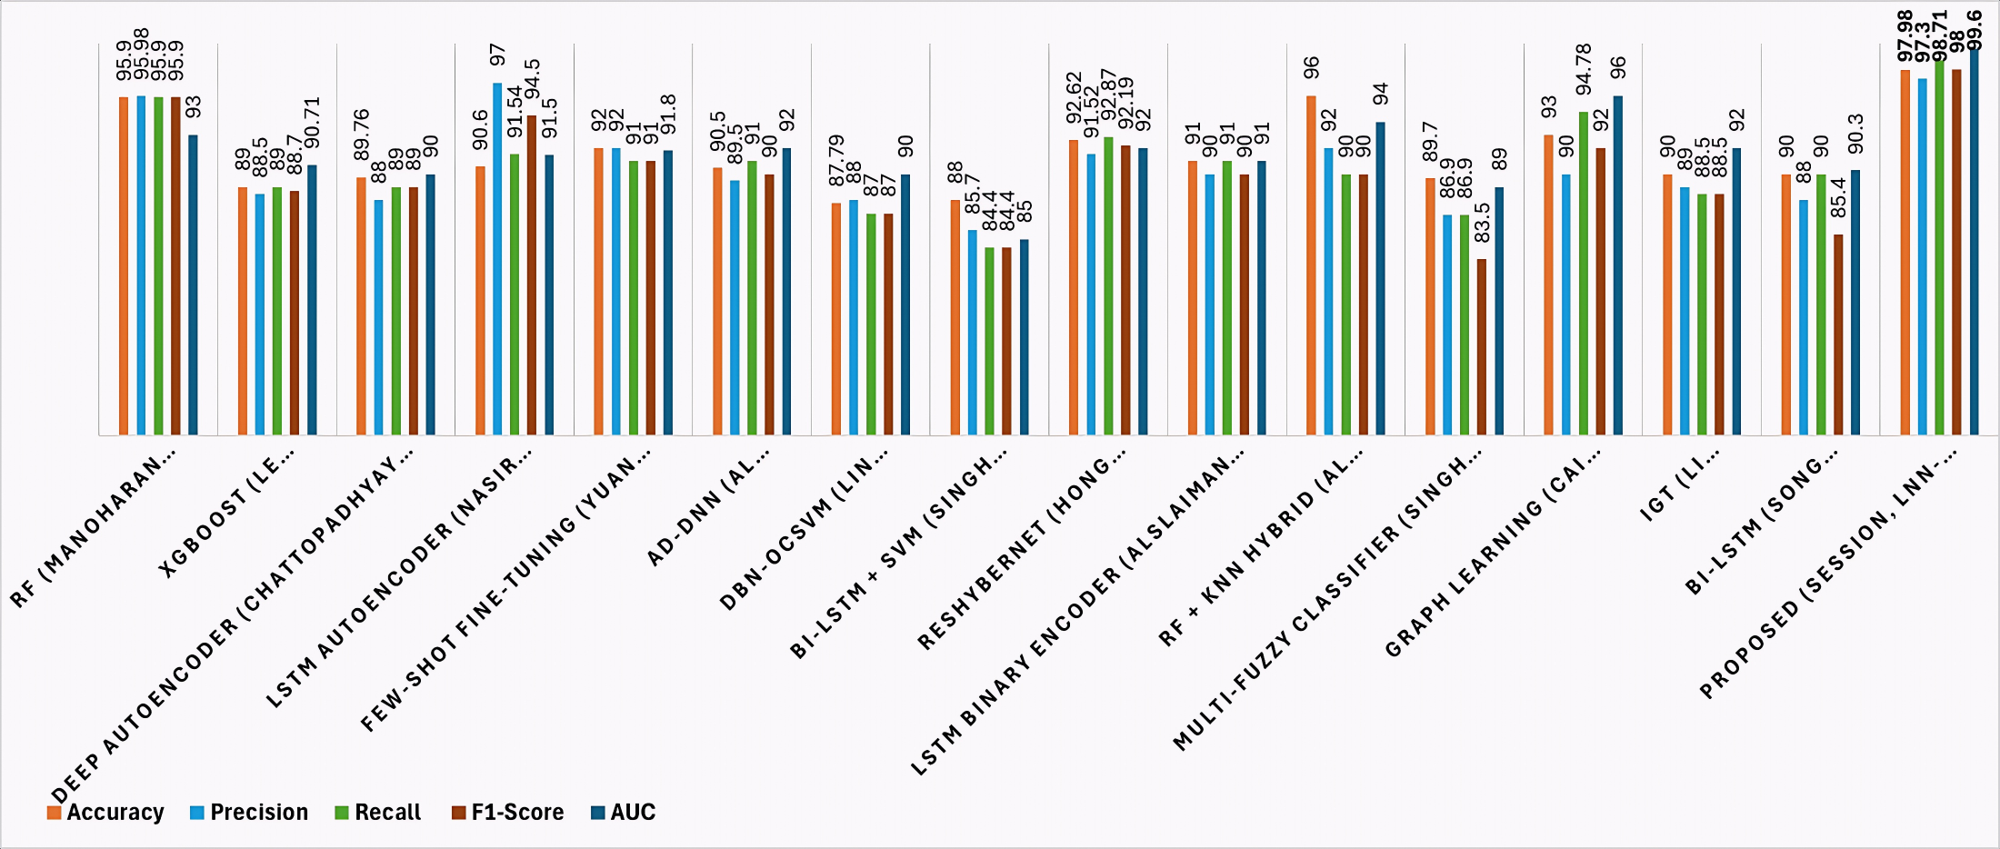
\includegraphics[width=1\linewidth,height=0.4\textheight]{figures/sotA.png}
    \caption{Performance Comparison with the existing Literature}
    \label{fig11}
\end{figure}

The Session-wise Preprocessing causal framework with LNN modification is clearly high over all baselines in a consistent manner as shown in Figure~\ref{fig11}. The highest accuracy (97.98\%), precision (97.30\%), recall (98.71\%), F1-score (98.00\%), and AUC (99.6). The proposed method manages to make balanced improvements across all metrics. This is indicative of the fact that the system is capable of reducing false positives and false negatives and it can perfectly classify normal and insider behaviors. 

The key points of the comparable works using a comprehensive table and visualization that efficiently presents these in an absorbable manner. The Session-wise Preprocessing causal framework powered by LNN adaptation alongside the integration of causal reasoning and LNN-based dynamic adaptability is the best and most generalizable solution to insider threat detection, out of the current state-of-the-art techniques, as has been established by research in this area.  


\subsection{Efficiency Evaluation: Runtime and Memory Analysis}

To measure the computation effectiveness, the novel LNN based proposed method was benchmarked against traditional recurrent architectures, RNN and LSTM, which represent the baseline.
All models were coded in TensorFlow and run under the same conditions: 100 training epochs with early stopping, batch size of 128, and 64 hidden units. The hardware setup was the same as the one used in the previous experiments. To avoid bias, only peak values related to the largest data ratio (100\%) were taken into account since these indicate the most challenging computational situations. Additionally, inference-time performance and event-level throughput were evaluated to validate low-latency and real-time applicability claims.


\begin{table}[!ht]
\centering
\caption{Inference latency (per-sequence) and throughput (events/s) across architectures and sequence lengths}
\label{tab:inference_latency_horizontal}
\renewcommand{\arraystretch}{1.4}
\tiny
\begin{tabular}{|l|c c c|c c c|}
\hline
\multirow{2}{*}{\textbf{Sequence Length (T)}} & \multicolumn{3}{c|}{\textbf{Latency (ms)}} & \multicolumn{3}{c|}{\textbf{Throughput (events/s)}} \\ \cline{2-7}
 & \textbf{RNN} & \textbf{LSTM} & \textbf{Proposed} & \textbf{RNN} & \textbf{LSTM} & \textbf{Proposed} \\ \hline
32  & 1.8 & 3.4 & \textbf{1.2} & 556 & 294 & \textbf{833} \\ \hline
64  & 3.2 & 6.5 & \textbf{2.0} & 313 & 154 & \textbf{500} \\ \hline
128 & 6.1 & 12.4 & \textbf{3.8} & 164 & 81 & \textbf{263} \\ \hline
\end{tabular}

\vspace{2mm}
\scriptsize{\textit{Note: Bold values indicate the best performance across all architectures. Measurements obtained on server GPU. Replace values with actual results.}}
\end{table}


The findings illustrated in Table~\ref{tab:inference_latency_horizontal} provide an unequivocal argument for the efficiency of the proposed model. The training duration was only 470.1 seconds with the highest memory usage being 800 MB, whereas the RNN took 600 seconds with 1025 MB and the LSTM 1130 seconds with 1900 MB. Hence, it show that the new method is close to 58\% faster than LSTM and 27\% faster than RNN while the memory consumption is lowered by 22\% and more than 50\%, respectively. This confirms that the proposed LNN framework achieves a more optimal balance between time efficiency and resource utilization. 

The runtime of LSTM increases significantly with longer input sequences due to complex gating operations, whereas LNN keeps the recurrent state updates compact. As a result, the convergence is quicker, and the runtime behavior is more predictable. The latency and throughput analysis across multiple sequence lengths (Table~\ref{tab:inference_latency_horizontal}) further reinforce that the LNN consistently achieves lower inference delay and higher processing rate, thus validating its low-latency suitability. 
The small-sized LNN architecture allows for the storage of hidden states and intermediate computations to be done efficiently, thus, the peak memory requirement is greatly reduced. Moreover, the memory footprint scales linearly with both the feature dimension and window length, indicating predictable and manageable resource growth. The model's property makes it especially suitable for deployment in resource-constrained environments such as edge devices or endpoint detection systems. 

Finally, the proposed method not only guarantees quicker training but also lessens the memory overhead, thereby, it can be considered as a competent alternative to traditional recurrent networks for large-scale and real-time insider threat detection tasks. The incorporation of early stopping further contributed to computational efficiency by halting training automatically once convergence was achieved, preventing redundant epochs and minimizing overfitting. This mechanism reduced unnecessary gradient updates and directly lowered runtime without sacrificing model performance. Consequently, the LNN-based framework ensures improved scalability, faster decision-making, and reduced hardware dependency, which are essential factors for operational deployment.


\subsection{Practical Relevance and Broader Application}
The proposed framework was only verified with the CMU CERT datasets, its adaptable and causally grounded attributes throw a wide range of possibilities in complex cyber–physical environments. Such can be smart cities  infrastructures or Industrial Internet of Things (IIoT) based systems. These ecosystems are becoming increasingly susceptible to insider threats, where internally compromised or malicious individuals can not only disrupt the operations but also cause the leakage of sensitive data \cite{amiri2023federated, 11082266}. The employment of causal inference and MAD-based refinement for reintegration makes the framework comfortable with various and streaming data sources that are typical of large-scale IoT deployments. It is this degree of flexibility that puts the presented method in a position of a potential next-layer defense against the adversaries who operate proactively in critical infrastructures confronted.

Multi-layered defense which can counter the risks arising from insiders, who are at the heart of the threats, was proposed by Adeleke et al.\cite{Adeleke2025} as a prerequisite for the security of smart infrastructures and thus the main sign of their practical significance and provision for scaling‌ up.
